% This must be in the first 5 lines to tell arXiv to use pdfLaTeX, which is strongly recommended.
\pdfoutput=1
% In particular, the hyperref package requires pdfLaTeX in order to break URLs across lines.

\documentclass[11pt]{article}

% Remove the "review" option to generate the final version.
\usepackage{acl}
\usepackage{amsmath}
\usepackage{graphicx}
\usepackage{subcaption}
\usepackage{booktabs}
\usepackage{url}

% Standard package includes
\usepackage{times}
\usepackage{latexsym}

% For proper rendering and hyphenation of words containing Latin characters (including in bib files)
\usepackage[T1]{fontenc}
% For Vietnamese characters
% \usepackage[T5]{fontenc}
% See https://www.latex-project.org/help/documentation/encguide.pdf for other character sets

% This assumes your files are encoded as UTF8
\usepackage[utf8]{inputenc}

% This is not strictly necessary, and may be commented out,
% but it will improve the layout of the manuscript,
% and will typically save some space.
\usepackage{microtype}

% If the title and author information does not fit in the area allocated, uncomment the following
%
%\setlength\titlebox{<dim>}
%
% and set <dim> to something 5cm or larger.

\title{Lab2 Report: End-to-End Speech Translation System Benchmarking}

\author{
  Team Jobless\\
  Jiyang Tang (jiyangta), Ran Ju (ranj), Tinglong Zhu (tinglonz), Xinyu Lu (xinyulu2)\\
}

\begin{document}
\maketitle


\section{Experimental Setup}

\subsection{Baseline}

The end-to-end speech translation architecture for our benchmark is an encoder-decoder model with multitask training objectives~\cite{inaguma2020espnet}.
During training, the encoder is trained with CTC loss~\cite{CTC} using source text as the ground truth, while the decoder, called \textit{MT decoder}, is trained using label smoothing cross-entropy loss using target text as the ground truth.
In addition, a separate transformer decoder sharing the same encoder connection called the \textit{ASR decoder}, is trained using label smoothing cross-entropy loss using source text as the ground truth.
Only the encoder and the MT decoder are used during inference.

To save time, we utilize a pre-trained model\footnote{\url{https://huggingface.co/espnet/brianyan918_mustc-v2_en-de_st_conformer_asrinit_v2_raw_en_de_bpe_tc4000_sp}} from Hugging Face Hub for our experiments.
This English-to-Dutch translation model contains a Conformer~\cite{conformer} encoder with $12$ layers and a Transformer~\cite{transformer} decoder with $6$ layers.
The encoder has a subsampling CNN layer with kernel size $31$, followed by identical Conformer blocks with $4$ attention heads and $2048$ hidden units.
The MT decoder blocks each contain $4$ attention heads and $2048$ hidden units.
Both the encoder and the decoder use a dropout rate of $0.1$ for positional encoding and attention.
The beam size is set to $10$ during inference.

\subsection{Evaluation}

BLEU (Bilingual Evaluation Understudy) measures the similarity of the machine-translated text to a set of reference texts.
It is a number between zero and one, and the higher the score is, the higher the quality the translation has.
Previous studies have shown that BLEU scores have a high correlation with human judgment~\cite{bleu} and it has become one of the canonical metrics for speech translation among the research community.
Thus, we use BLEU scores to represent the quality of our translation models.

\subsection{Data}

We use the test set from MuST-C~\cite{mustc} for evaluating our models.
For each language pair, MuST-C contains hundreds of hours of audio recordings from English TED talks and sentence-level transcriptions and translations.
Considering the model size and inference speed, we selected $20$ samples from the English-to-Dutch test set to calculate our benchmarking metrics.


\subsection{Benchmarking}

For benchmarking, we measure the latency in seconds, FLOPs, and BLEU scores for each experiment and visualize the results.
For latency, we measure the time it takes to perform inference on every test sample and take the average of them except the first one.
We rely on the DeepSpeed~\cite{deepspeed} library for FLOPs calculation.
Specifically, we measure the total FLOP count for translating all samples and take the average to mitigate the effect of varying input audio lengths.
However, since the DeepSpeed FLOP profiler only works on CUDA devices, we have to run experiments to calculate FLOPs separately using an Nvidia V100 16GB GPU instead of only the CPU.

Except for FLOPs calculation, all experiments are conducted using a laptop CPU under the same conditions.
We stopped as many applications and background services as possible before benchmarking.
The hardware specification is shown below:
\begin{enumerate}
    \item Laptop: Dell G15 5511
    \item CPU
    \begin{enumerate}
        \item 11th Gen Intel i7-11800H, 2.30GHz
        \item Speed 3.35 GHz
        \item 8 cores, 16 logical processors
        \item L1 cache: 640 KB
        \item L2 cache: 10.0 MB
        \item L3 cache: 24.0 MB
    \end{enumerate}
    \item Memory: 32GB, dual-channel DDR4
    \item OS: Windows 10 Education 22H2, OS Build 19045.3570
    \item Python environment:
    \begin{enumerate}
        \item Python==3.10
        \item PyTorch==1.12.1
        \item ESPnet==202308
    \end{enumerate}
    \item Test data is loaded into memory beforehand.

\end{enumerate}

All experiments are conducted using ESPnet~\cite{espnet,inaguma2020espnet}. Since each sample has different durations and output lengths, there will exist some variance between latencies from different samples.

\section{Varying Input Size}
The first way we vary the input size is to change the hop length. The larger the hop length, the smaller the input size. The hop length for each experiment is shown in Table \ref{tab:vary_input_size}. 

The experiment results are shown in Figure \ref{fig:input_size}. From the BLEU score vs FLOPs plot we observe that as we decrease the input size, the FLOPs decrease as expected. As the FLOPs decrease, we don't see a clear trend of increasing or decreasing BLEU scores. We think the reason is that we didn't re-train the model after changing the hop length. Since the model is trained using a hop length of 160, inference with different hop lengths will affect and bring a lot of uncertainty to the BLEU score performance. 

The BLEU score vs latency graph looks similar to the BLEU score vs FLOPs one. The latency decreases as we decrease the input size. The BLEU score generally decreases as we change the input size because of the different input sizes used to train and infer the model, but there is no specific trend observed. 

For the relationship between FLOPs and latency, we find that generally as the FLOPs increase, the latency increases as well. However, for the original and input\_size1 experiments, the relationship is the opposite. From original to input\_size1, we increase the hop length by 40, which is slightly smaller than the difference between input\_size2 and input\_size3. We hypothesize the reason is that it is related to the way the hardware deals with memory optimization. 

The second way that we vary input size is to first decrease the sample rate from 16k to 8k and then increase the hop length to decrease the input size, and the hop length hyperparameters are in Table~\ref{tab:vary_input_size}. The experiment results are shown in Figure~\ref{fig:input_size_method2}. By examining the graph depicting the relationship between BLEU score and FLOPs, it becomes apparent that reducing the input size leads to the expected decrease in FLOPs. However, as FLOPs decrease, there isn't a discernible pattern of either an increase or a decrease in the BLEU score. The graph illustrating the relationship between BLEU score and latency closely resembles the one comparing BLEU score to FLOPs. As the input size decreases, latency also decreases. The BLEU score tends to decrease when adjusting the input size due to disparities between the training and inference input sizes, although there isn't a clear, consistent trend observed. When examining the connection between FLOPs and latency, we generally observe that as FLOPs increase, latency also tends to increase.

The difference between the two methods is that the first one only changes the hop length while the second one decreases the sample rate before increasing the hop length. We choose these two methods to understand how changing hop length and sample rate affects the latency and BLEU score. In terms of the BLEU score, we observe that if we decrease the sample rate by half, the BLEU score drops dramatically, except input\_size2, the BLEU scores for all other models drop to less than 10. We think the reason is that the dropped samples contain important context information for the model to understand. In terms of latency, we find that if we decrease the sample rate first, the latency will decrease significantly. It is as expected due to there is less computation. In all, we think decreasing the sample rate is not a good strategy for decreasing the input size since the BLEU score drops too much. In comparison, changing hop length directly has a better trade-off between performance and latency. 

\begin{table}
\centering
\small
\begin{tabular}{cc}
\toprule  
\textbf{Model} & \textbf{Hop length}\\
\midrule 
original & 160\\
input\_size1 & 200\\
input\_size2 & 250\\
input\_size3 & 300\\
\bottomrule
\end{tabular}
\caption{Experiments of Varying Input Size}
\label{tab:vary_input_size}
\end{table}

\begin{figure*}[h]
    \centering
    \begin{subfigure}{0.32\textwidth}
        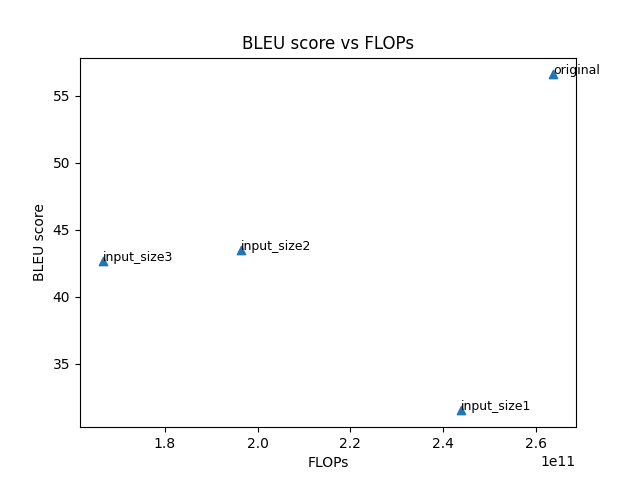
\includegraphics[width=\textwidth]{images/input_size/BLEU_vs_FLOP.png}
        \caption{FLOPs vs. BLEU}
    \end{subfigure}
    %\hfill % adds horizontal space between the images
    \begin{subfigure}{0.32\textwidth}
        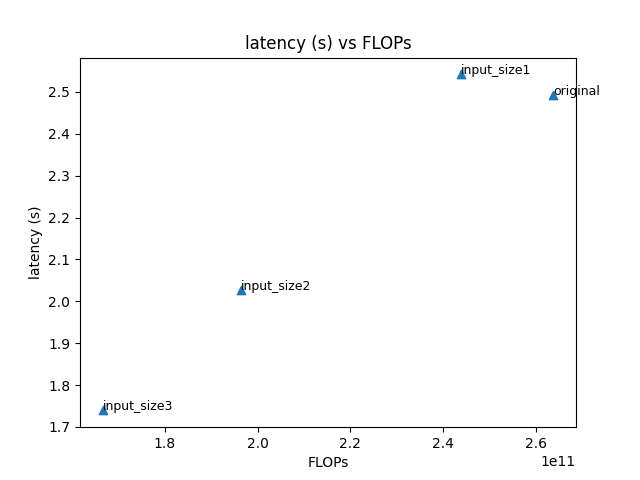
\includegraphics[width=\textwidth]{images/input_size/latency_vs_FLOP.png}
        \caption{FLOPs vs. Latency}
    \end{subfigure}
    %\hfill % adds horizontal space between the images
    \begin{subfigure}{0.32\textwidth}
        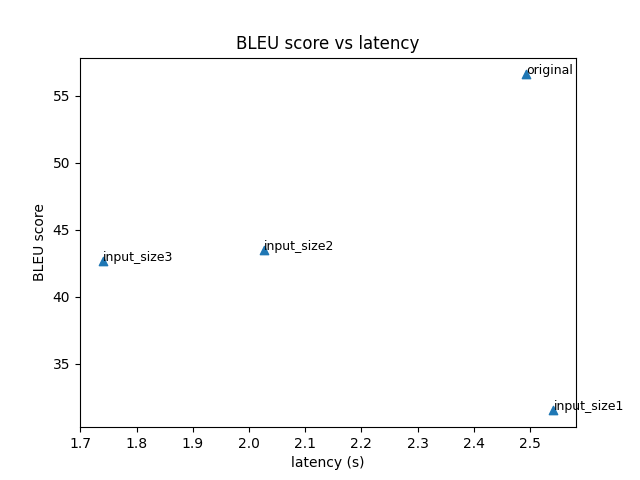
\includegraphics[width=\textwidth]{images/input_size/BLEU_vs_latency.png}
        \caption{Latency vs. BLEU }
    \end{subfigure}
    \caption{\label{fig:input_size}Comparative Plots For Different Input Size (Method 1)}
\end{figure*}


\begin{figure*}[h]
    \centering
    \begin{subfigure}{0.32\textwidth}
        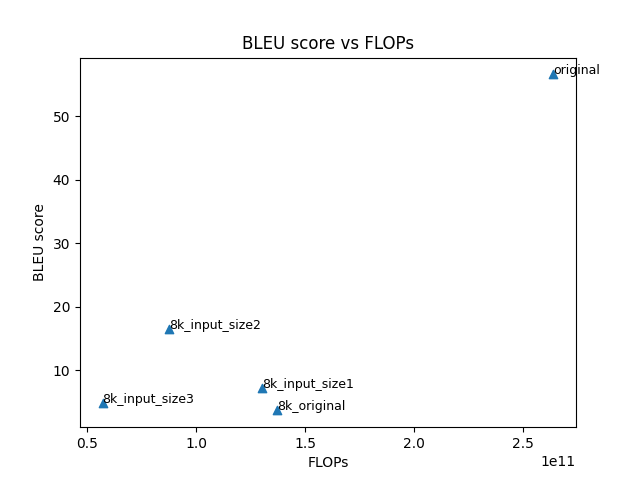
\includegraphics[width=\textwidth]{images/input_size_method2/BLEU_vs_FLOP.png}
        \caption{FLOPs vs. BLEU}
    \end{subfigure}
    %\hfill % adds horizontal space between the images
    \begin{subfigure}{0.32\textwidth}
        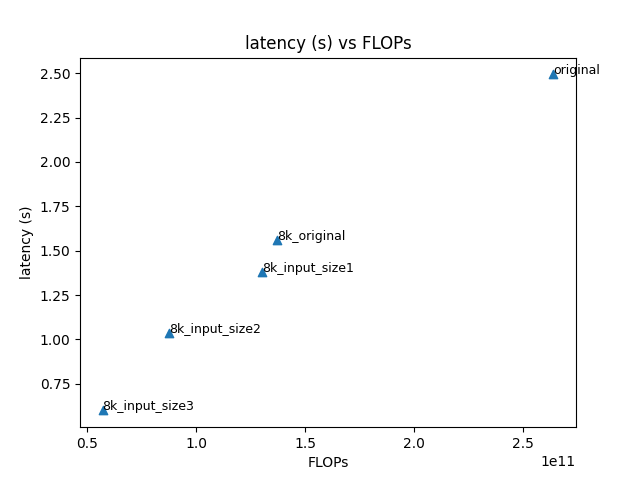
\includegraphics[width=\textwidth]{images/input_size_method2/latency_vs_FLOP.png}
        \caption{FLOPs vs. Latency}
    \end{subfigure}
    %\hfill % adds horizontal space between the images
    \begin{subfigure}{0.32\textwidth}
        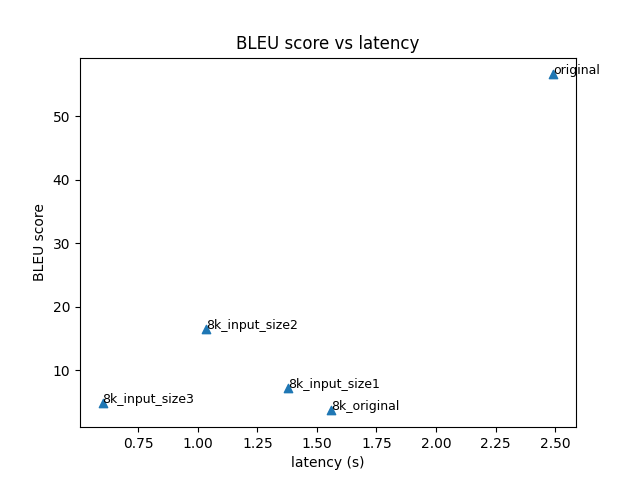
\includegraphics[width=\textwidth]{images/input_size_method2/BLEU_vs_latency.png}
        \caption{Latency vs. BLEU }
    \end{subfigure}
    \caption{\label{fig:input_size_method2}Comparative Plots For Different Input Size (Method 2)}
\end{figure*}

\section{Varying Model Size}

\begin{figure*}[!h]

    \centering
    \begin{subfigure}{0.322\textwidth}
        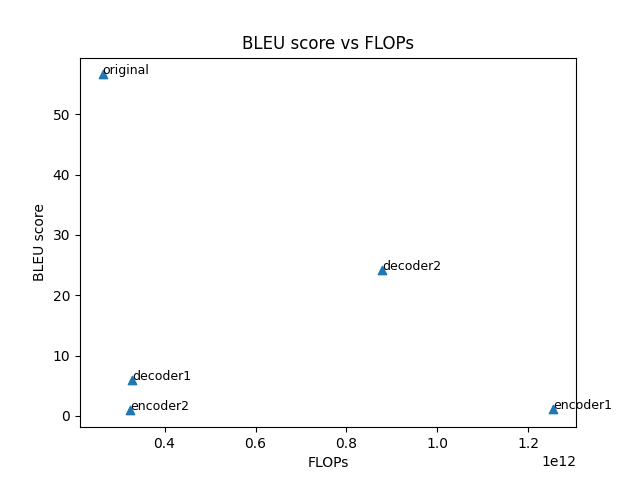
\includegraphics[width=\textwidth]{images/model/BLEU_vs_FLOP.png}
        \caption{FLOPs vs. BLEU}
    \end{subfigure}
    % \hfill % adds horizontal space between the images
    \begin{subfigure}{0.32\textwidth}
        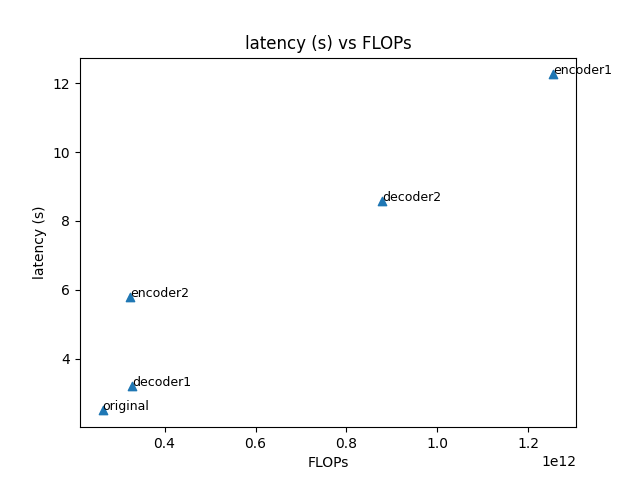
\includegraphics[width=\textwidth]{images/model/latency_vs_FLOP.png}
        \caption{FLOPs vs. Latency}
    \end{subfigure}
    % \hfill % adds horizontal space between the images
    \begin{subfigure}{0.32\textwidth}
        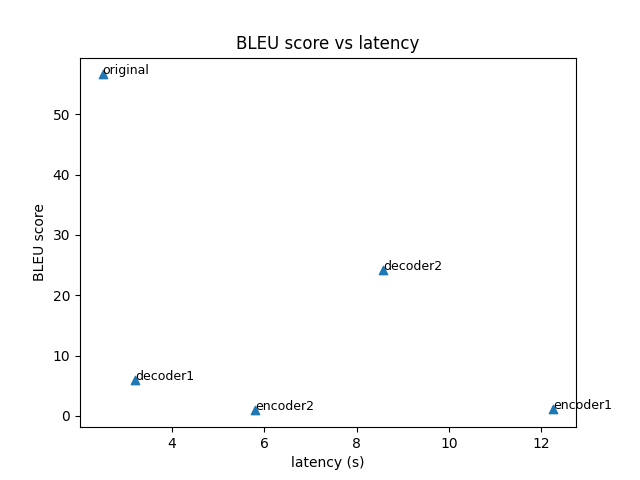
\includegraphics[width=\textwidth]{images/model/BLEU_vs_latency.png}
        \caption{Latency vs. BLEU }
    \end{subfigure}
    \caption{\label{fig:model_size}Comparative Plots For Different Model Size}  
\end{figure*}

Modifying a pre-trained model's architecture can drastically alter its performance. Table \ref{tab:model_parameters} shows the experiments we conducted to adjust model parameters.
% \begin{itemize}
%   \item decoder1: 
%   \begin{align*}num\_blocks&=4\end{align*}
%   \item decoder2: \begin{align*}
%     attention\_heads&=2 \\
%     linear\_units&=1024
% \end{align*}
%   \item encoder1:  \begin{align*}num\_blocks&=8\end{align*}
%   \item encoder2: \begin{align*}
%   output\_size&=128\\
%     attention\_heads&=2 \\
%     linear\_units&=1024
% \end{align*}
% \end{itemize}


\begin{table*}[h]
    \centering
    \resizebox{0.95\linewidth}{!}{
    
    \begin{tabular}{lccccc}
        \toprule
        Model & $num\_blocks$ & $attention\_heads$ & $linear\_units$ & $output\_size$ & \textbf{Total} parameter count \\
        \midrule
        Original (Encoder) & 12 & 4 & 2048 & 256 & 57,592,032 \\
        Original (Decoder) & 6 & 4 & 2048 & -- & 57,592,032 \\
        \midrule
        decoder1 & 4 & -- & -- & -- & 54,434,528 \\
        decoder2 & -- & 2 & 1024 & -- & 54,440,160 \\
        encoder1 & 8 & -- & -- & -- & 47,033,568 \\
        encoder2 & -- & 2 & 1024 & 128 & 18,918,368 \\
        \bottomrule
    \end{tabular}
    
    }
    \caption{Parameter settings for different models compared to original ESPNet parameters. -- indicates that the parameter retains its original value.}
    \label{tab:model_parameters}
\end{table*}

\begin{enumerate}
    \item \textbf{Reducing Layer Depth and Widths}

To reduce the layer depth, we reduced the number of blocks with decoder1 and encoder1.
Specifically, we keep the first $N$ layers and discard subsequent ones.
In addition, we reduce the width of the entire model reducing the output size of both the encoder and the decoder in encoder2 experiment.
Decreasing the model size reduces the capability of the model to recognize complex patterns while drastically cutting down the computational cost and parameter count.

\item \textbf{Reducing Number of Attention Heads}

In decoder2 and encoder2. we adjusted attention\_heads and linear\_units. In this way, we lessen the model's capacity to focus on various parts of the input sequence in parallel while narrowing the model width.

In these ways, we reduce the parameters and maintain the already learned features as much as possible at the same time. All the methods aim to minimize the computational burden.
\end{enumerate}

The results are shown in Figure \ref{fig:model_size}. From the result, we could see that the model with the lowest FLOPs(decoder1) does not have the lowest BLEU score. decoder2 shows a relatively high BLEU score with intermediate FLOPs, indicating a good trade-off between computational complexity and model performance. decoder1 has a relatively low latency and moderate BLEU score which could be advantageous in real-time applications where lower latency is critical. encoder1 and encoder2 seem to be ineffective. 

Our explanations are:
\begin{itemize}
  \item When reducing model size without retraining, the pre-existing weights might not be optimal for the new architecture. It could lead to nonsensical outputs from the decoder.
  
  \item The decoder relies on its previous outputs so without proper adaptation to the reduced size architecture, it could generate "garbage" outputs, repeating or elongating translations.

  \item To mitigate the problems, we should reduce the model's size coupled with retraining, fine-tuning, layer pruning, or employing knowledge distillation techniques.

\end{itemize}




\section{Putting it together}

\begin{table}[h]
    \centering
    \resizebox{0.98\linewidth}{!}{
    
    \begin{tabular}{lccc}
        \toprule
        Model & BLEU scores & Latency (s) & FLOPs \\
        \midrule
        Original & \textbf{56.6} & 2.5 & 263,773,099,929 \\
        \midrule
        encoder1 & 1.2 & 12.3 & 1,254,943,585,484 \\
        encoder2 & 0.9 & 5.8 & 324,969,515,078 \\
        decoder1 & 6.0 & 3.2 & 329,232,078,169 \\
        decoder2 & 24.2 & 8.6 & 878,961,158,694\\
        \midrule
        input\_size1 & 31.5 & 2.5 & 243,909,508,076 \\
        input\_size2 & 43.5 & 2.0 & 196,505,325,796 \\
        input\_size3 & 42.6 & 1.7 & 166,594,033,230 \\

        8k\_input\_size1 & 7.3 & 1.4 & 130,435,959,142 \\
        8k\_input\_size2 & 16.5 & 1.0 & 87,710,174,390 \\
        8k\_input\_size3 & 4.9 & \textbf{0.6} & \textbf{57,216,657,598} \\
        \bottomrule
    \end{tabular}
    
    }
    \caption{Benchmarking results for all experiments.}
    \label{tab:model_parameters}
\end{table}

Here, we did not conduct experiments that combine different input sizes and model sizes. Reducing the model sizes without fine-tuning and retraining will lead to huge and unacceptable performance degradation (e.g. senseless sentences, repeating a single token/words until reaching the maximum length, etc.). If we reduce the model size and input size at the same time, the results will get worse. Thus, we did not combine different input sizes and model sizes in this section, but we did put the results corresponding to different input sizes and model sizes together for analysis (Table \ref{fig:all_together}).

From the scatter plots below, we can see that reducing the input sizes (by increasing the hop length of MFCC) can help dramatically improve the latency and FLOPs while keeping a merely acceptable performance degradation. One possible explanation for this could be speech signals are periodic signals, the semantic information contained in a period may be the same. Since increasing the hop length will not lead to a huge information loss, the reduction of input sizes also has little risk of repeating the outputs until reaching the maximum output length. Thus, increasing the hop length of MFCC features may not lead to a huge information loss but can help reduce the latency since the number of frames the encoder has to deal with is only half of that of the original. But directly downsampling the waveform will cause dramatic performance degradation; this might be due to the losing information from part of the frames in the raw waves. In comparison, increasing hop length can reduce input size while keeping an acceptable information loss since it gets information from all frames in the raw waves. 

\begin{figure*}[h!]
    \centering
    \begin{subfigure}{0.32\textwidth}
        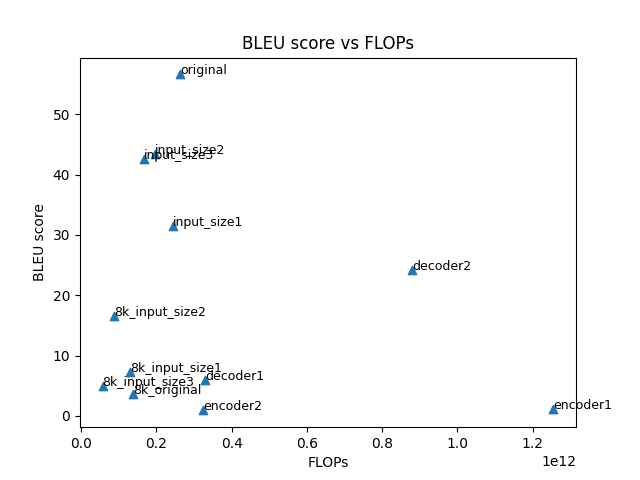
\includegraphics[width=\textwidth]{images/All/BLEU_vs_FLOP.png}
        \caption{FLOPs vs. BLEU (all together)}
    \end{subfigure}
    % % \hfill % adds horizontal space between the images
    \begin{subfigure}{0.32\textwidth}
        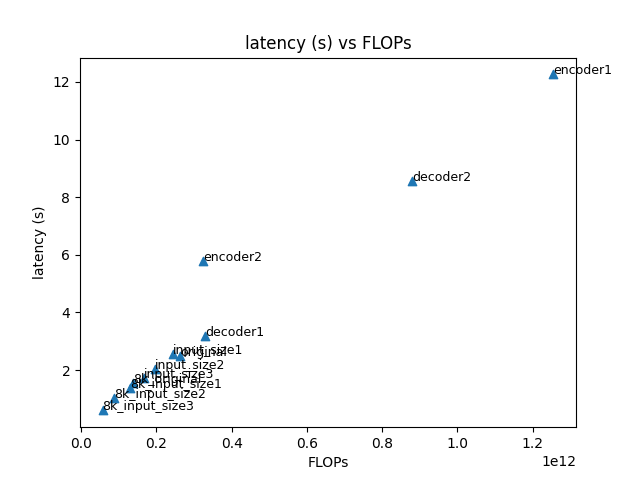
\includegraphics[width=\textwidth]{images/All/latency_vs_FLOP.png}
        \caption{FLOPs vs. Latency (all together)}
    \end{subfigure}
    % \hfill % adds horizontal space between the images
    \begin{subfigure}{0.32\textwidth}
        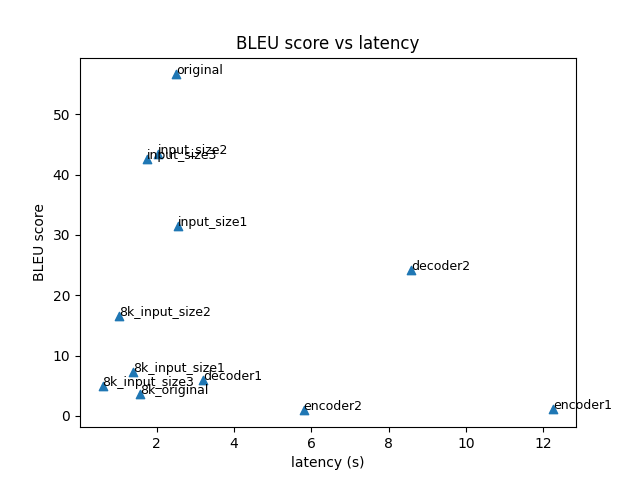
\includegraphics[width=\textwidth]{images/All/BLEU_vs_latency.png}
        \caption{Latency vs. BLEU (all together)}
    \end{subfigure}
    \caption{\label{fig:all_together}Comparative Plots (All together)}     
\end{figure*}
However, when we tried to decrease the model size, the performance dropped dramatically (no matter whether we reduced the size of the encoder or the decoder). As we only keep the first few layers of the encoder/decoder, we will lose the semantic insights from the latter layers, which are important for translation. In addition, as mentioned above, losing semantic information will cause the model to repeatedly generate the same tokens/words, which will not only decrease its performance but will also greatly increase its inference latency.

In short, if we want to improve the model inference latency without having serious performance degradation and without retraining the model, increasing MFCC's hop length to 300 would be a good solution.



\bibliography{custom}
\bibliographystyle{acl_natbib}


\end{document}
